\section{Problem Statement}

First, some notation used in the rest of the paper.

Our goal is to take the user's complaints about the current state
of the database, and identify transformations over the database
query log that, when applied to the database, ``fixes'' these
complaints.  Although the general formulation of the problem that
we will introduce is intractable, we will reduce the scope of the
problem to a useful and tractable version.  To begin, we will
introduce the notation that is used in the rest of the paper.

\stitle{Def 1 (Database, State, Query)}: Let a database
be defined as the result of applying a sequence of queries in the query log
$Q_{seq}=\{Q_1,..., Q_n\}$ to an initial database $D_0$.  
Applying the query log to the initial database 
results in $n$ intermediate database states $\{D_i = Q_i(D_{i-1}) | i \in [1, n]\}$.  
where $D_n = Q_{seq}(D_0) = Q_n(\ldots Q_1(D_0))$ is the current state of the database. 
We assume that a subset of the query log has been replaced with {\it corrupted queries} 
such that $D_n$ and $Q_{seq}$ differ from the true database state $D^*_n$ and query log $Q^*_{seq}$.

In our current problem, we only deal with non aggregation and non-join queries.
In addition, for ease of exposition, we assume that the database contains a single table $T$ 
($T^*$ in the true database) containing $m$ numerical attributes $a_1,\ldots,a_m$, 
where the primary key is $a_1$.  
In Section~\ref{blah}, we will describe how our techniques extend to multi-table databases.



\stitle{Def 2 (Complaints and Complaint Sets)}:
The tuple-wise difference between two databases $D_1$ and $D_2$ can be viewed as a patch
$P_{D_1, D_2}$ that contains {\it difference pairs} $(t_i \in T, t^*_i \in T^*)$.
The non-null entries represent tuple modifications, whereas a null entry for $t_i$ ($t'_i$) represent a tuple addition (deletion) to $D_n$.
Similar to source code patches, patches can be applied to a database $P(D_n) = D^*_n$.

The user provides a {\it complaint set} $C$ that specify the perceived incorrect tuples in $D_n$.
$C$ is simply a patch.
We define a complete complaint set when $C = P_{D_n, D^*_n}$.
In contrast, an {\it incomplete complaint set}  may contain complaints that are false negatives (insertions that should be in $C$ but are not),
false positives (deletions that are not present), and errors (proposed value of a $t'$ is incorrect).

The accuracy of an incomplete complaint set can be measured by the ratio $acc_C = \frac{|C \cap \Delta|}{|\Delta|}$.


\begin{figure}[h]
\centering
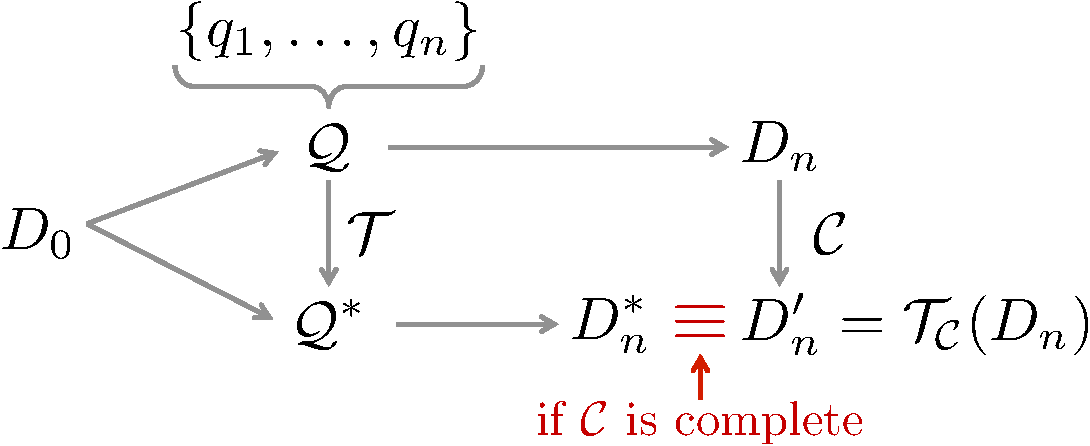
\includegraphics[width = 2in]{figures/probtransform}
\caption{Graphical depiction of the general XXX problem.}
\label{f:probtransform} 
\end{figure}



\stitle{Problem Statement}: The most general version of the problem
(depicted in Figure~\ref{f:probtransform}) is to find a sequence of
transformations $T$ that insert, delete, and/or modify queries in $Q_{seq}$ 
such that the resulting sequence, $Q^'_{seq} = T(Q_{seq})$, resolves the user's complaint set. 

However this problem is ill-defined because there exist an unbounded set of transformations that
can resolve the user's complaint set.  A naive solution is to append to the query log a statement
that deletes all the records in the database, followed by a query that insert all of the correct records.
Unfortunately this naive solution does not help explain the complaints in any way!

For this reason, we constrain the set of possible transformations $\mathcal{T}$,
and define a metric evaluate the quality of a transformation.
\xxx{define $\mathcal{T}$ here.}

%\xxx{understand how different than materialized view/query synthesis}.

In this paper, we describe solutions to three versions of this problem.

\begin{problem}[Prob-Complete]\label{prob:complete}
Given $C = P_{D_n, D^*_n}$, $Q_{seq}$, and the sequence of database states $D_0,\ldots,D_n$, 
identify a sequence of transformations $T$ such that:
\begin{CompactItemize}
\item $T(Q_{seq})(D_0) = C(D_n)$
\item $|T| = 1$
\item $T$ metric is minimized
\end{CompactItemize}
\end{problem}

This variation of the problme relaxes the constraint that the complaint set must be complete, and allows
for both false positives as well as false negatives.  The goal is the same, however the constraints are relaxed:

\begin{problem}[Prob-Incomplete]\label{prob:incomplete}
Given $C$ where $acc_C < 1$, $Q_{seq}$, and the sequence of database states $D_0,\ldots,D_n$, 
identify a sequence of transformations $T$ such that:
\begin{CompactItemize}
\item $T(Q_{seq})(D_0) = D^*_n$
\item $T$ metric is minimized.
\item $|T| = 1$
\end{CompactItemize}
\end{problem}

Finally, we extend the problem to allow transformations with one or more operations.

\begin{problem}[Prob-MultiQ]\label{prob:multi}
Given $C$ where $acc_C < 1$, $Q_{seq}$, and the sequence of database states $D_0,\ldots,D_n$, 
identify a sequence of transformations $T$ such that:
\begin{CompactItemize}
\item $T(Q_{seq})(D_0) = D^*_n$
\item $T$ metric is minimized.
\end{CompactItemize}
\end{problem}



 Given a database D, its initial
state D0, a sequence of queries Qseq={Q1,..., Qm}and the corresponding
states {D1,..., Dm}, a complete(incomplete) complaint set  Con Dm
(that changes the state of D to Dm*), we want a transformation
(delete/swapping/update), T, changes Qseqto Qseq* such that the
final state of D change from Dmto Dm*. We say  Qseq*is optimal when
diff( Qseq, Qseq*) is minimized.


\subsection{Basic Formulation}


\subsubsection{A Naive Approach}


\subsection{Extensions}

\subsubsection{Incomplete Complaints}

\subsubsection{Multi-query Resolution}


